This chapter discusses in detail the organization and internal structure of the code that is the implementation of the novel algorithms discussed in Chapter \ref{chp:cosy}. For reference, a reproduction of the code itself may be found in Appendix~\ref{apx:code}. First, the user input is discussed. Next, the \textit{cosy.fox} level of the code is examined. Finally, the structure of the FORTRAN code is briefly considered. Figure~\ref{fig:cosy_flowchart} is referenced during these discussions.

In addition to the user's input file, COSY also uses a \textit{cosy.fox} file. This file contains a plethora of global variables, functions, and routines which the user can access. However, \textit{cosy.fox} can also be used to hide most of the complicated machinery from the user. For example, for this study the routine in \textit{cosy.fox} transforms the COSY coordinates $(x, a, y, b, \ell, d)$ into absolute coordinates $(x, p_x, y, p_y, t, E)$,\footnote{Recall from Eq. \eqref{eqn:phaseSpaceVector} that $x$ and $y$ are the transverse coordinates; $a=p_x/p_0$ the $x$ angle; $b=p_y/p_0$ the $y$ angle; $\ell=-(t-t_0)v_0\gamma/(1+\gamma)$ the time-of-flight in units of length; $\delta=(K-K_0)/K_0$ the relative energy; $E$ the total energy; $K$ the kinetic energy; and the subscript $0$ denotes the coordinate of the reference particle.} and then relays the information to the FORTRAN code. Both the user file and the \textit{cosy.fox} file are written in COSYScript, the programming language of COSY. 

\begin{figure}[!htb]
  \centering
    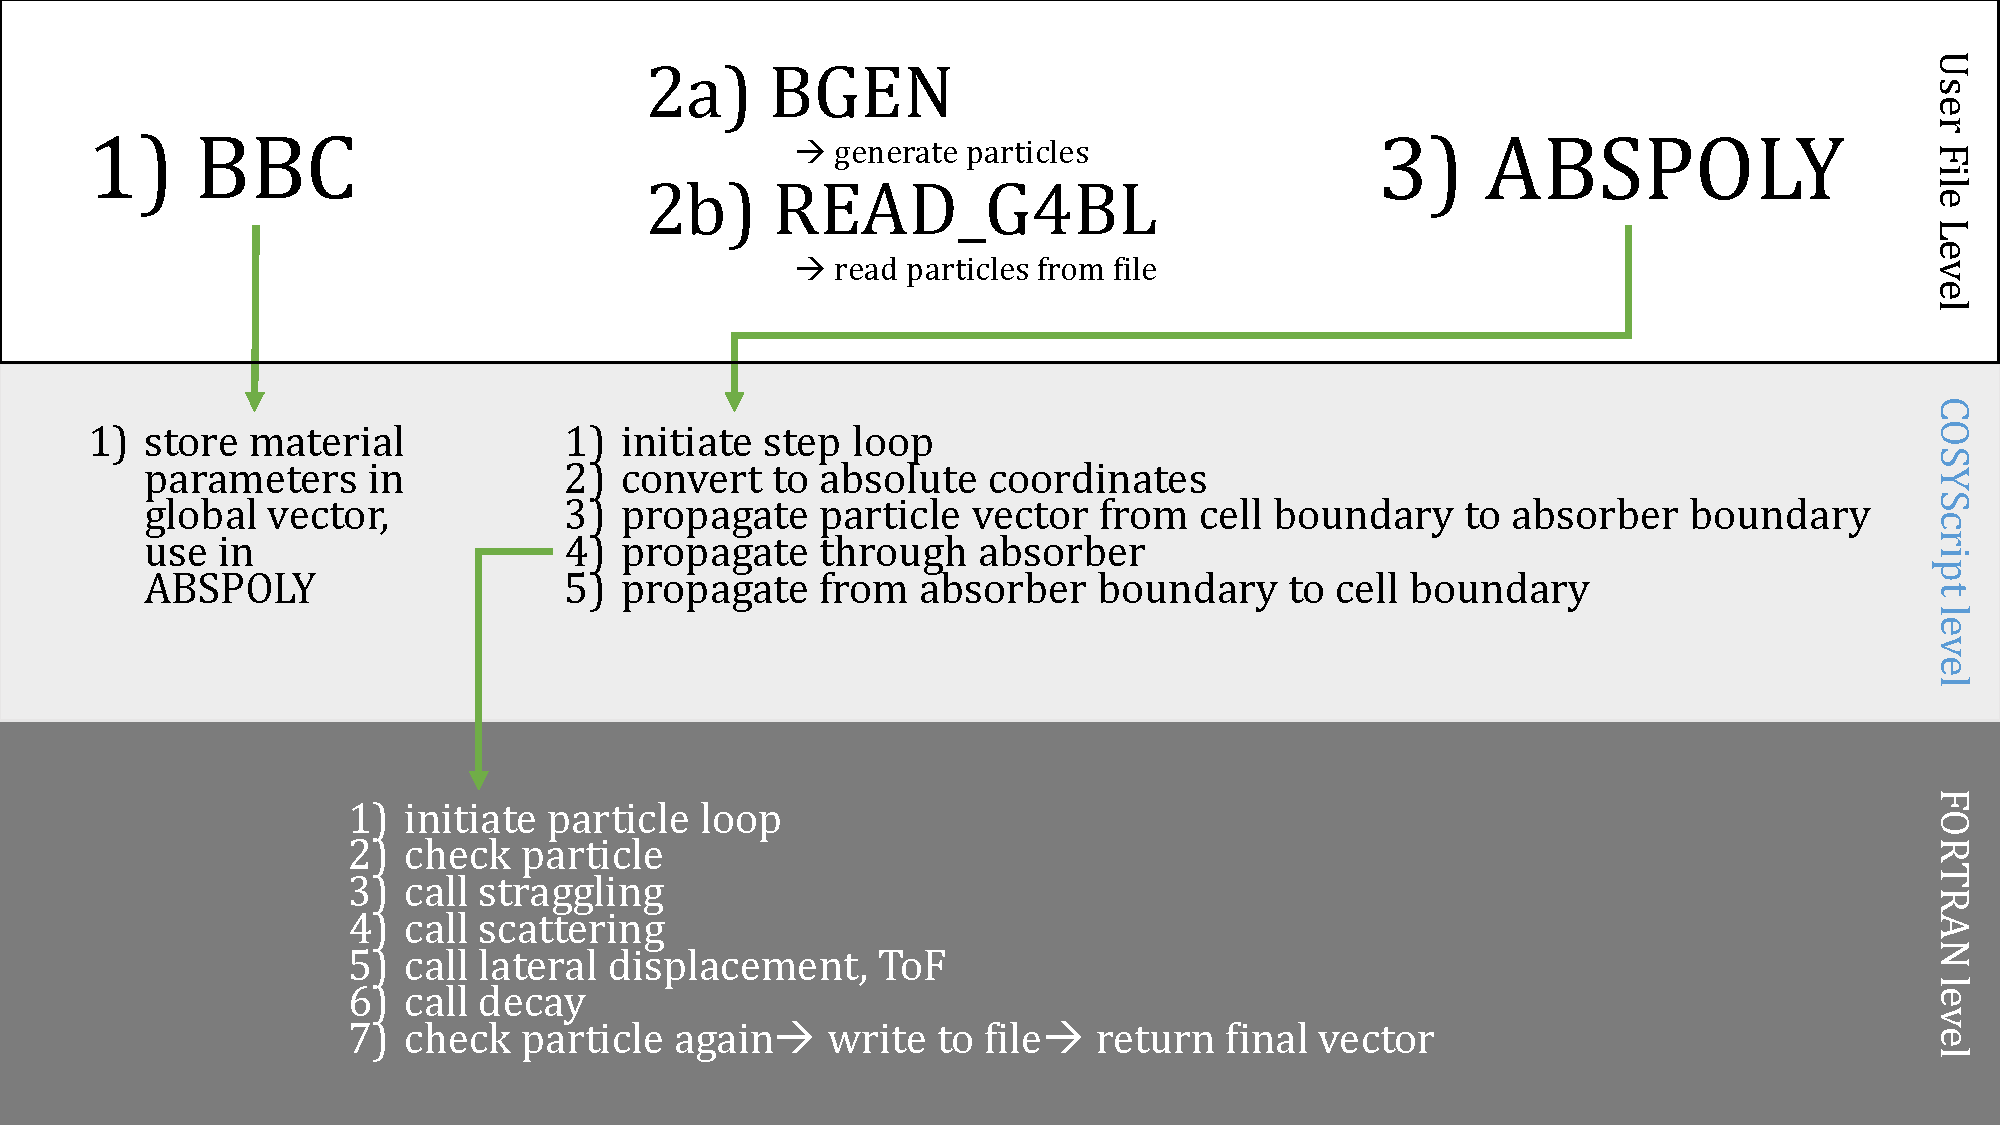
\includegraphics[width=\textwidth]{Figures/cosy_flowchart} 
  \caption{A flowchart for the structure of the new COSY routines implemented in this work.}
  \label{fig:cosy_flowchart}
\end{figure}

\Section{User Input}\label{ssc:user_input}

As with the deterministic absorber routine previously present in COSY, \texttt{WA}, the user must first call the procedure\\
\texttt{BBC} <$Z$> <$A$> <$\rho$> <$I$> <$\delta$> <$C$> \texttt{;} \\
This stores the material parameters in a global array. The arguments are the nuclear charge $Z$, the atomic mass $A$, the density of the material $\rho$, the ionization energy $I$, the density correction $\delta$, and the shell correction $C$. Next, the user must either generate a distribution of particles or read a distribution of particles from a file. Using \\
\texttt{BGEN} <$n$> <$V$> <$\mu_x$> <$\sigma_x$> <$\mu_{p_x}$> <$\sigma_{p_x}$> <$\mu_y$> <$\sigma_y$> <$\mu_{p_y}$> <$\sigma_{p_y}$> <$\mu_t$> <$\sigma_t$> <$\mu_{p_z}$> <$\sigma_{p_z}$> \texttt{;}\\
the user can generate a Gaussian beam of $n$ particles into a 2D vector $V$. Note that in COSY, a 2D vector is a vector of vectors and is not the same data class as an array. Alternatively, the user may use \\
\verb|READ_G4BL| <\texttt{file}> <$n$> <$V$> \texttt{;}\\
to read an ASCII-formatted G4Beamline file of $n$ particles and store it into a 2D vector $V$. Finally, the user can call\\
\texttt{ABSPOLY} <$S_1$> <$S_2$> <$n$> <$L$> <$A$> <$V$> <$X_0$> <$S_n$> <$L_c$> <$O$> \texttt{;}\\
where $S_1$\footnote{For a full description of the entrance and exit polynomials $S_1$ and $S_2$, please see the COSY beam physics manual \cite{cosy}, page 33.} is an $n^{th}$ order polynomial describing the entrance surface, $S_2$ is an $n^{th}$ order polynomial describing the exit surface, $L$ is the on-axis length of the absorber, $A$ is the aperture, $V$ is the 2D input and output particle vector, $X_0$ is the radiation length of the material, $S_n$ is the number of steps inside the absorber, $L_c$ is the length of the absorber cell, and $O$ is the output unit number (e.g. ``12'' to save the results in \texttt{fort.12}). A depiction of some of the parameters can be found in Figure~\ref{fig:abspoly}.

\begin{figure}[!htb]
  \centering
    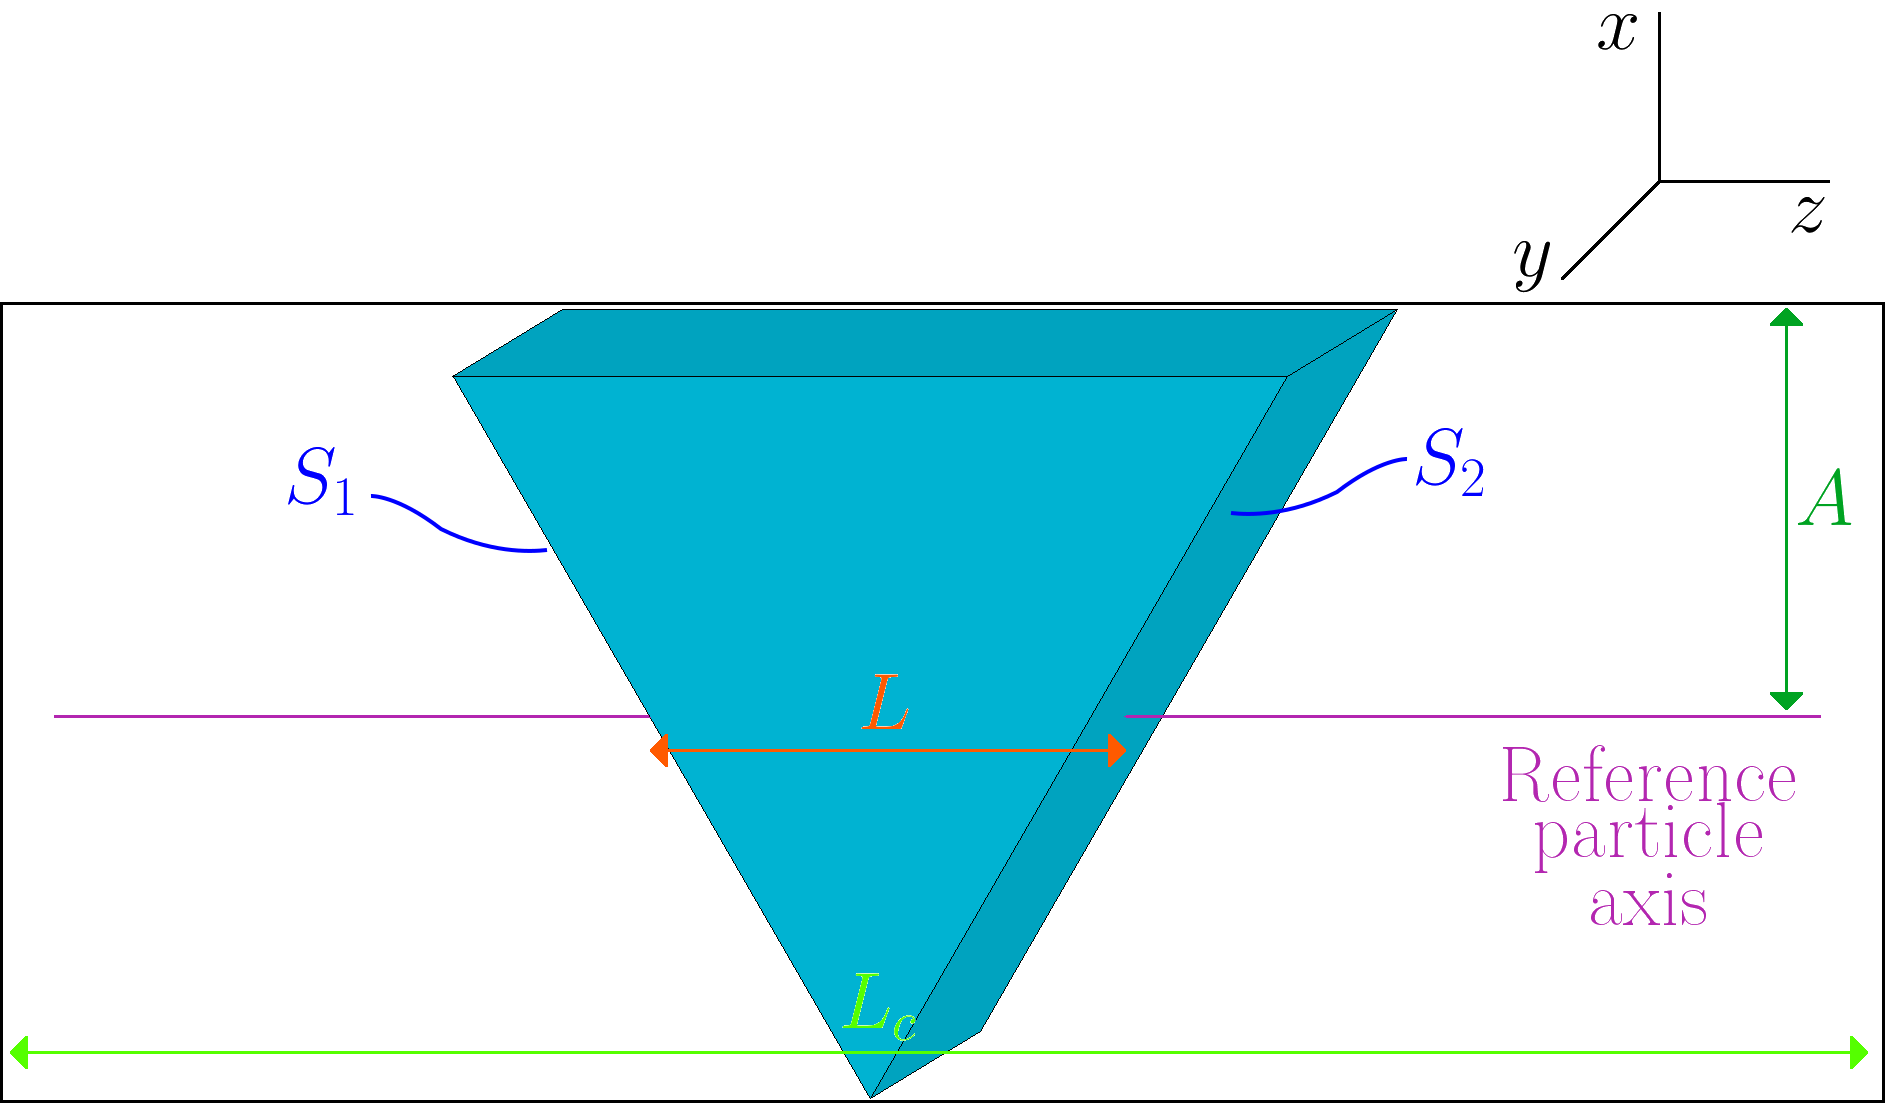
\includegraphics[width=\textwidth]{Figures/abspoly} 
  \caption{Cartoon example of some of the \texttt{ABSPOLY} parameters.}
  \label{fig:abspoly}
\end{figure}

\Section{COSYScript Level}\label{ssc:cosyscript}

As previously mentioned, the \texttt{ABSPOLY} routine is defined in the external file \textit{cosy.fox}. Here, if the user desires iteration through the absorber, the step loop over $S_n$ is initialized. Next, input 2D vector $V$ is converted from coordinates relative to the reference particle to absolute coordinates. The particle vector is then propagated from the cell boundary (whose width is defined by $L_c$) to the absorber (whose on-axis width is defined by $L$). If $L_c<L$ then no propagation occurs. When the particles are at the absorber boundary, the 2D particle vector $V$ is passed on to the FORTRAN level of the code, where propagation through the absorber takes place. The routine linking the COSYScript and FORTRAN levels is \texttt{STOABS} and is discussed in Section~\ref{ssc:fortran}. After the 2D particle vector $V$ is returned, $V$ is propagated to the end of the cell and returned to the user.

\Section{FORTRAN Level}\label{ssc:fortran}

Except for the propagation of particles through the absorber, the processes found in Section~\ref{ssc:cosyscript} are much faster in COSYScript than in FORTRAN. This is because processes like coordinate conversion, propagation through a vacuum, etc. are deterministic and can therefore be handled by transfer maps.

The routine\\
\texttt{STOABS} <$V$> <$m$> <$L$> <$MP$> <$X_0$> <$O$> <$A$> <$n$> \texttt{;} \\
takes input parameters from the COSYScript level and returns the input 2D particle vector $V$. Here, $m$ is the particle mass (taken from the reference particle), $L$ is an $n$-dimensional array containing the path lengths for each particle, $MP$ is an array containing the material parameters (taken from the global array $BETHEBLOCHC$ set up by the routine \texttt{BBC}), $X_0$ is the radiation length of the material, $O$ is the output unit number, $A$ is the aperture, and $n$ is the number of particles.

Once the FORTRAN level has this information, a loop over $n$ particles is started. Each particle is checked at the beginning of each loop for the following flags: particle stopped, particle hit aperture, particle missed absorber, drift. If either the particle was stopped ($E\leq m$) or the particle hit the aperture ($x^2+y^2\geq A^2$) then the particle is terminated. If the particle missed the absorber completely then the drift flag is turned on. If the drift flag is on then the particle is simply propagated without the stochastic processes called.

Provided that the particle has not been flagged, the particle is subject to energy straggling and then multiple scattering. After these two routines, the lateral displacement and time-of-flight corrections are called. It should be noted that the order matters for energy straggling and multiple scattering. The order does not matter for lateral displacement and time-of-flight provided that both straggling and scattering have already occurred. Finally, decay can be called. Note that for this work, decay has been turned off completely, and so this step is skipped.

Finally, the particle is checked again. If the output unit number $O$ is not equal to zero then the particles are written to a file. Lastly, the 2D particle vector $V$ is returned to the COSYScript level.

\Section{Summary}

Figure~\ref{fig:cosy_flowchart} displays the conceptual process of operating the implemented routines. First, the user defines the material parameters in \texttt{BBC}, which stores these parameters as global variables at the COSYScript level. Next, the user creates a 2D vector of particles, either by generating a Gaussian beam via \texttt{BGEN} or reading particles from a G4Beamline file via \verb|READ_G4BL|. Finally, the user calls the \texttt{ABSPOLY} routine. \texttt{ABSPOLY} converts the COSY coordinates to and from absolute coordinates and calls the FORTRAN routine to step through the absorber. At the FORTRAN level, each particle is subjected to the energy straggling, multiple scattering, transverse displacement, and time-of-flight algorithms described in Chapter \ref{chp:cosy}. These particles are returned to the user at the end of the propagation.